\section{Introduzione}
L'obiettivo di questo elaborato è la presentazione di un approfondimento per l'esame di sicurezza informatica che consiste nel'implementare 
un attacco padding Oracle contro un algoritmo di cifratura a blocchi in modalità CBC.
L'algoritmo di cifratura a blocchi scelto è il DES con chiave a 64bit ma potrebbe funzionare anche 
su algoritmi più complessi come AES con chiave a 128bit purchè usati in modalità CBC.
\section{CBC Mode}

CBC (Cipher Block Chaining) è una modalità di cifratura a blocchi, questo significa che il testo in chiaro viene cifrato passando blocchi di bytes di una 
lughezza predefinita alla funzione di cifratura. Se però ogni blocco fosse cifrato indipendentemente senza ulteriori manipolazioni uno stesso 
input genererebbe uno stesso cifrato in output, per questo nella modalità CBC (figura \ref{fig:cbc_enc}), i blocchi non sono cifrati indipendentemente ma 
l'output della cifratura del blocco precedente viene messo in Xor con il testo in chiaro generando molta più differenza fra gli output.
Dato l'input di questo tipo di modalità è necessario utilizzare un vettore di inizializzazione (IV) random o fisso al primo blocco da cifrare, in questo progetto viene usato 
un vettore di inizializzazione random.

\begin{figure}[h!]
    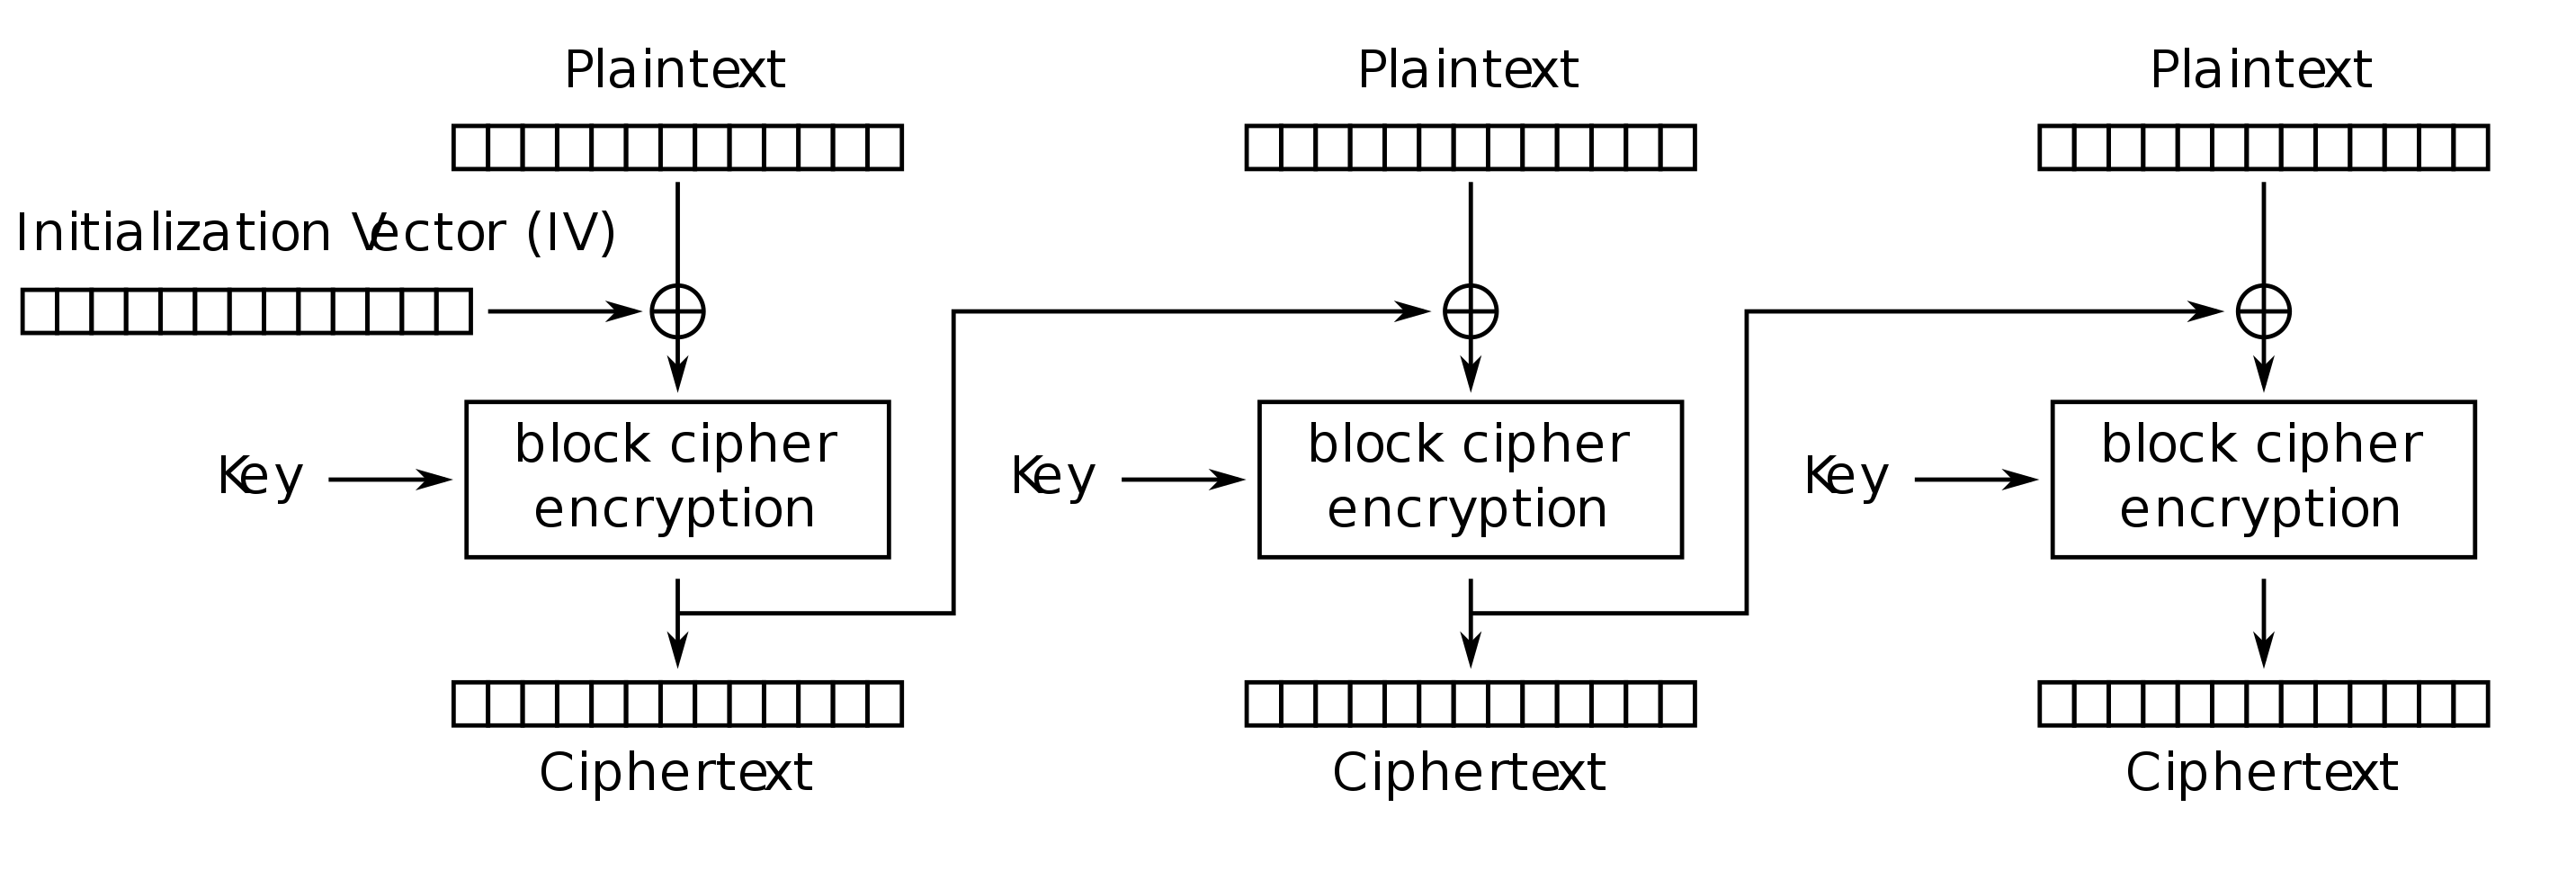
\includegraphics[width=0.7\textwidth]{img/CBC_encr.png}
    \centering
    \caption{CBC modalità cifratura}
    \label{fig:cbc_enc}
\end{figure}

per quanto riguarda la decifratura del messaggio (figura \ref{fig:cbc_decr}), sarà sufficiente eseguire l operazione inversa mettendo in Xor il cifrato del blocco precedente con l output della funzione di decifratura, utilizzando lo stesso vettore di inizializzazione (IV).

\begin{figure}[h!]
    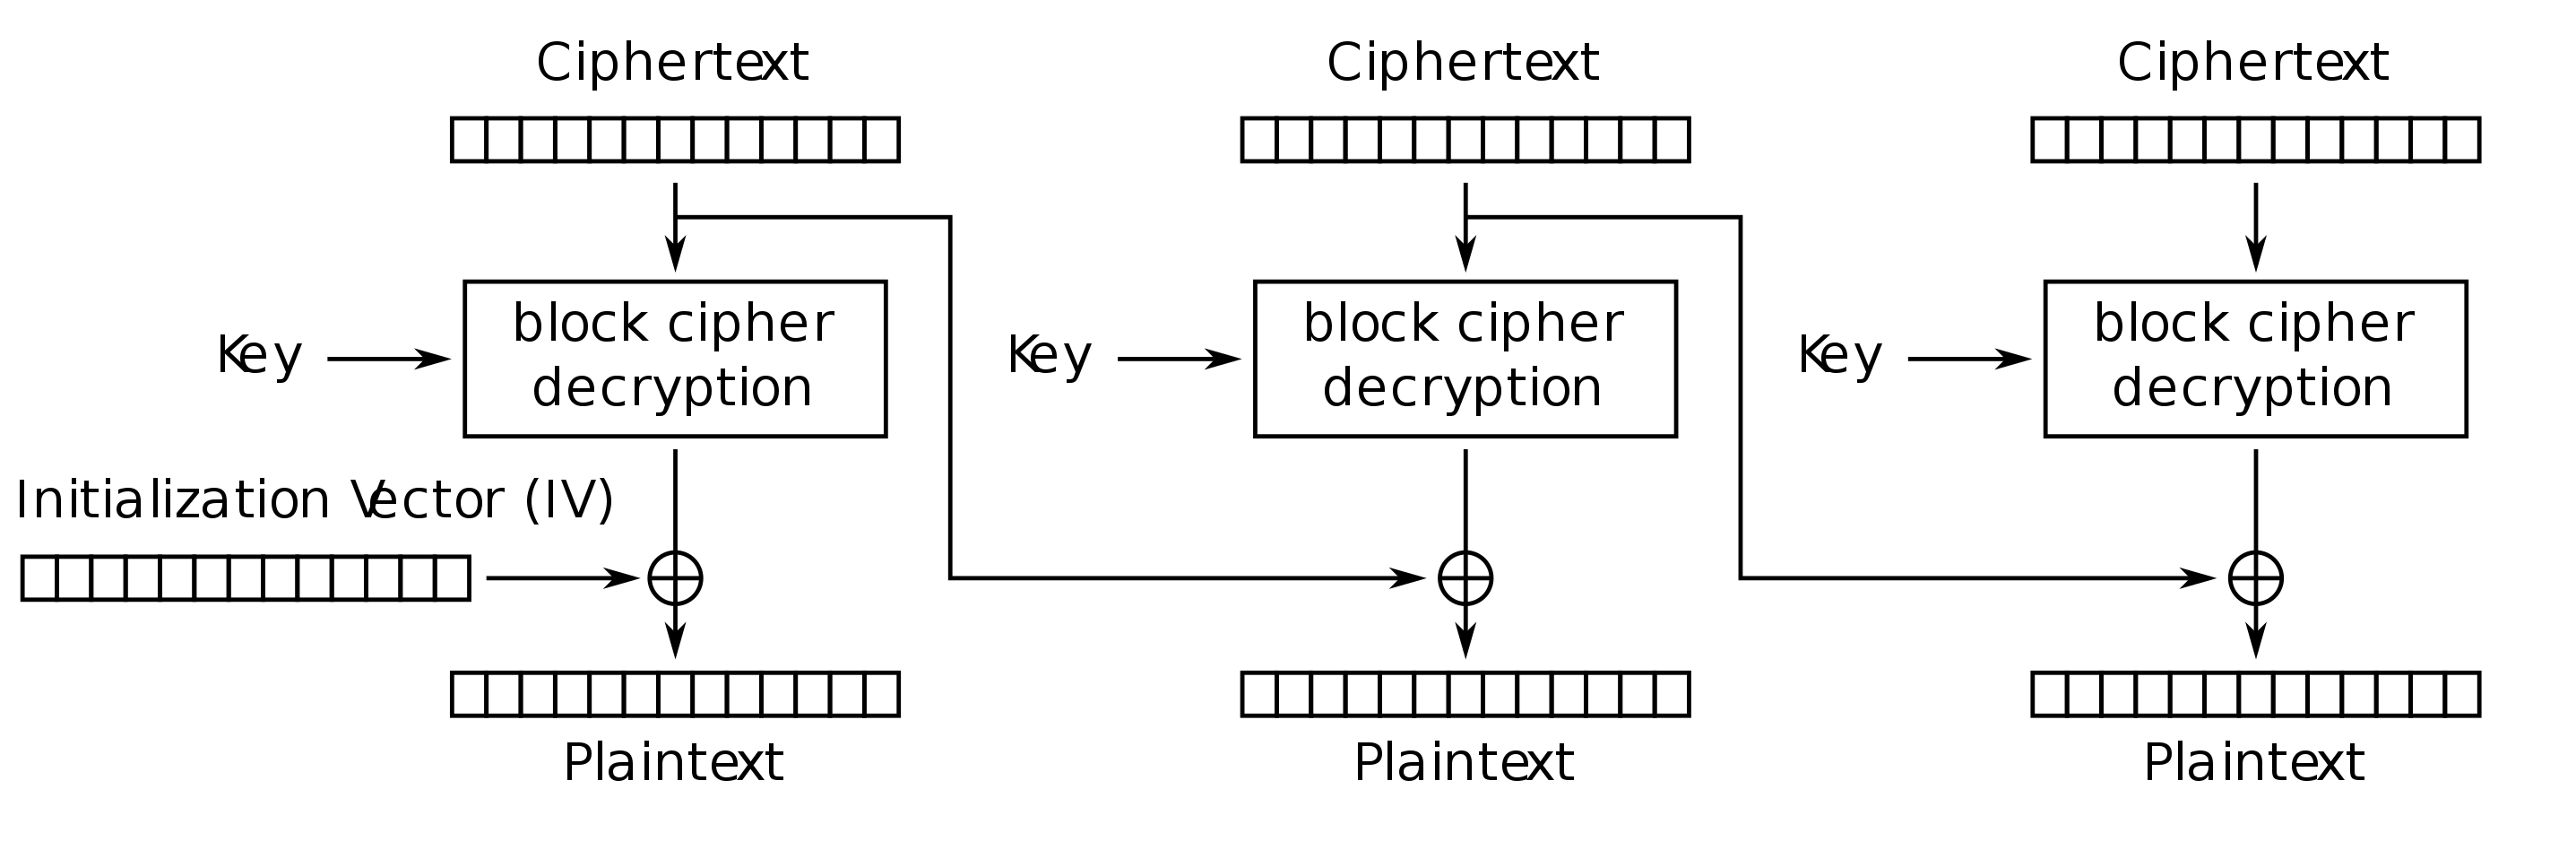
\includegraphics[width=0.7\textwidth]{img/CBC_decr.png}
    \centering
    \caption{CBC modalita decifratura}
    \label{fig:cbc_decr}
\end{figure}

\section{DES}
DES è un aloritmo di cifratura a chiave simmetrica, ovvero che usa la stessa chiave sia per cifrare che decifrare, 
la chiave deve essere scambiata su un canale sicuro dalle due parti coinvolte.
Lavora con blocchi in input di dimensione fissa da 64bit che tramite una serie di operazioni di trasformazione vengono 
portati in testo cifrato della stessa lunghezza
\section{Padding}
La cifratura a blocchi richiede una lunghezza fissa in ingresso ma i messaggi da cifrare 
. non sono tutti di dimensioni multiple alla dimensione del blocco accettato dall'algoritmo di cifratura. 
Per questo all'ultimo gruppo di bytes che non rispetta la dimensione viene aggiunto del padding finale.
Ci son diversi tipi di padding, quello che implementa DES è PKCS\#5 and PKCS\#7, che consiste nell aggiungere n bytes con valore pari al numero di bytes da aggiungere per arrivare alla dimensione del blocco. 
\\Quindi per esempio:

\begin{verbatim}
    01
    02 02
    03 03 03
    04 04 04 04
    05 05 05 05 05
    ...
\end{verbatim}
Questo metodo di padding supporta blocchi con massima lunghezza di 256byte, perchè un byte può rappresentare valori da 0 a 255.
Per esempio nel caso di DES dove la dimensione del blocco è di 64bit (8byte), un padding sarebbe:

\begin{verbatim}
    ... | AA AA AA AA AA AA AA AA | AA AA AA AA AA 03 03 03 |
\end{verbatim}
Nel caso in cui il massaggio sia invece di un multplo esatto della lunghezza dei blocchi, per evitare di fare controlli aggiuntivi se il padding c'è o no, viene agiunto ugualmente un blocco intero di padding. In Questo modo in fase di decifratura il padding sarà sempre presente e sempre da rimuovere.
\section{Attacco padding Oracle}

L'attacco consiste nello sfruttare informazioni provenienti dalla correttezza del padding di un messaggio creato ad hoc.
L'abilità di poter dare informazioni sulla correttezza del padding è data dal padding oracle che è un elmemento 
fondamentale dell'attacco senza il quale non è possibile procedere.
In (figura \ref{fig:attack_1}) è rappresenato un esempio di decifratura che aiuterà a spiegare la dinamica dell'attacco.
Per semplicità di rappresentazione vengono usati blocchi da 4 bytes ma il ragionamento può essere esteso a n bytes di blocchi.
I blocchi denominati con Dx rappresentano lo stato intermedio dopo la decifratura ma prima di eseguire l operazione di Xor, l' attacco si basa sul trovare proprio questo stato intermedio questo perchè:

\begin{verbatim}
   D = C ^ P 
   and 
   P = C ^ D
\end{verbatim}
C è conosciuto perchè è il testo cifrato, quindi trovato D possiamo ricavare il testo in chiaro P.

\begin{figure}[h!]
    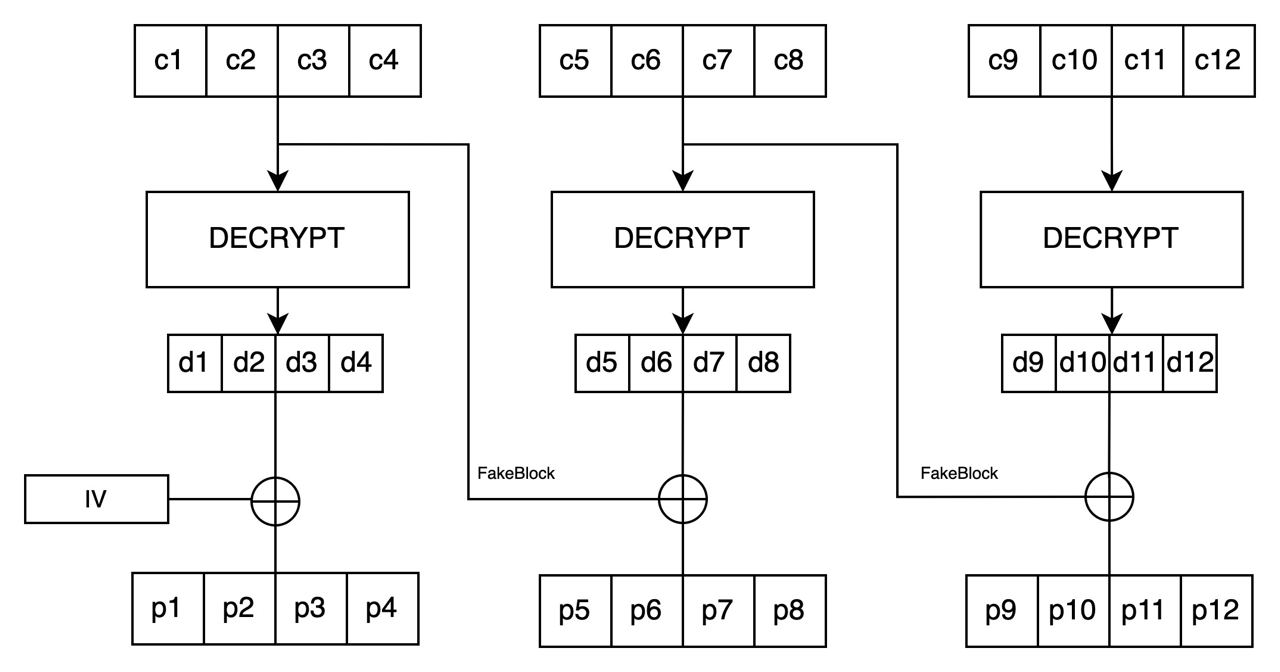
\includegraphics[width=0.8\textwidth]{img/attack.jpeg}
    \centering
    \caption{Spiegazione attacco}
    \label{fig:attack_1}
\end{figure}

\subsection{Manipolazione della cifratura}
Il padding oracle passato qualsiasi testo cifrato ci dirà se il padding è corretto o no, quindi ipotizzando di avere un padding 0x01 a P12 (P'12)
proviamo a trovare per quale byte a C8 otteniamo risposta positiva dal padding oracle.
Nella pratica (figura \ref{fig:attack_2}), facciamo variare da 0 a 255 il valore di C8, chiamandolo C'8, finchè il padding 
oracle non da risposta positiva, a quel punto abbiamo che:
\begin{verbatim}
    D12 = C'8 ^ P'12 
 \end{verbatim}
 \begin{figure}[h!]
    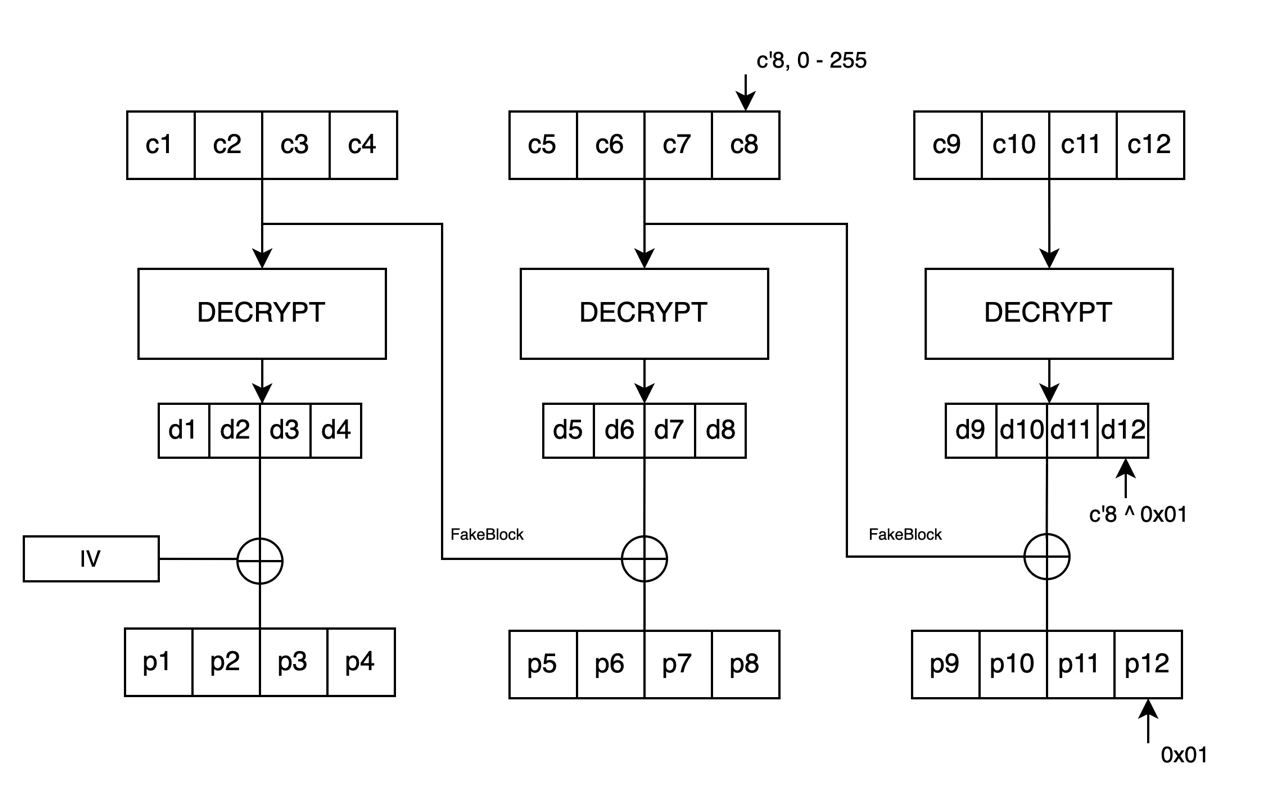
\includegraphics[width=0.8\textwidth]{img/attack_first_byte.jpeg}
    \centering
    \caption{Attacco al primo byte}
    \label{fig:attack_2}
\end{figure}
abbiamo trovato il valore di D, possiamo quindi procedere a trovare il l'effettivo valore di P12:
 \begin{verbatim}
    P'12 = D12 ^ C'8

    ma
    D12 = C8 ^ P12

    quindi

    P'12 = C8 ^ P12 ^ C'8
 \end{verbatim}
 Abbiamo che C8 è il byte originale del testo cifrato, C'8 il byte al quale il padding oracle ha risposto correttamente e P'12 il padding che abbiamo ipotizzato 0x01
 \begin{verbatim}
    P12 = C8 ^ 0x01 ^ C'8
 \end{verbatim}
abbiamo trovato il primo byte di testo in chiaro.
\subsection{Byte Successivi}
Il ragionamento che è stato fatto per un byte può essere ripotrato ai byte successivi, cambiando il padding corrispondente al numero di byte che sto manipolando.
Qundi nella pratica ora ipotizzo che il penultimo byte del testo in chiaro abbia padding 0x02 e cerco per quale valore c'7 iniettato al padding oracle da risposta corretta.
Nel fare questa operazione però va cambiato anche il valore di c8 perchè deve corrispondere ad un padding corretto, e in questo caso il padding corretto lo 
si ha avendo anche p12 a 0x02, possedendo il valore di d12 però possiamo facilmente ricavare il corretto valore di c8
\begin{figure}[h!]
    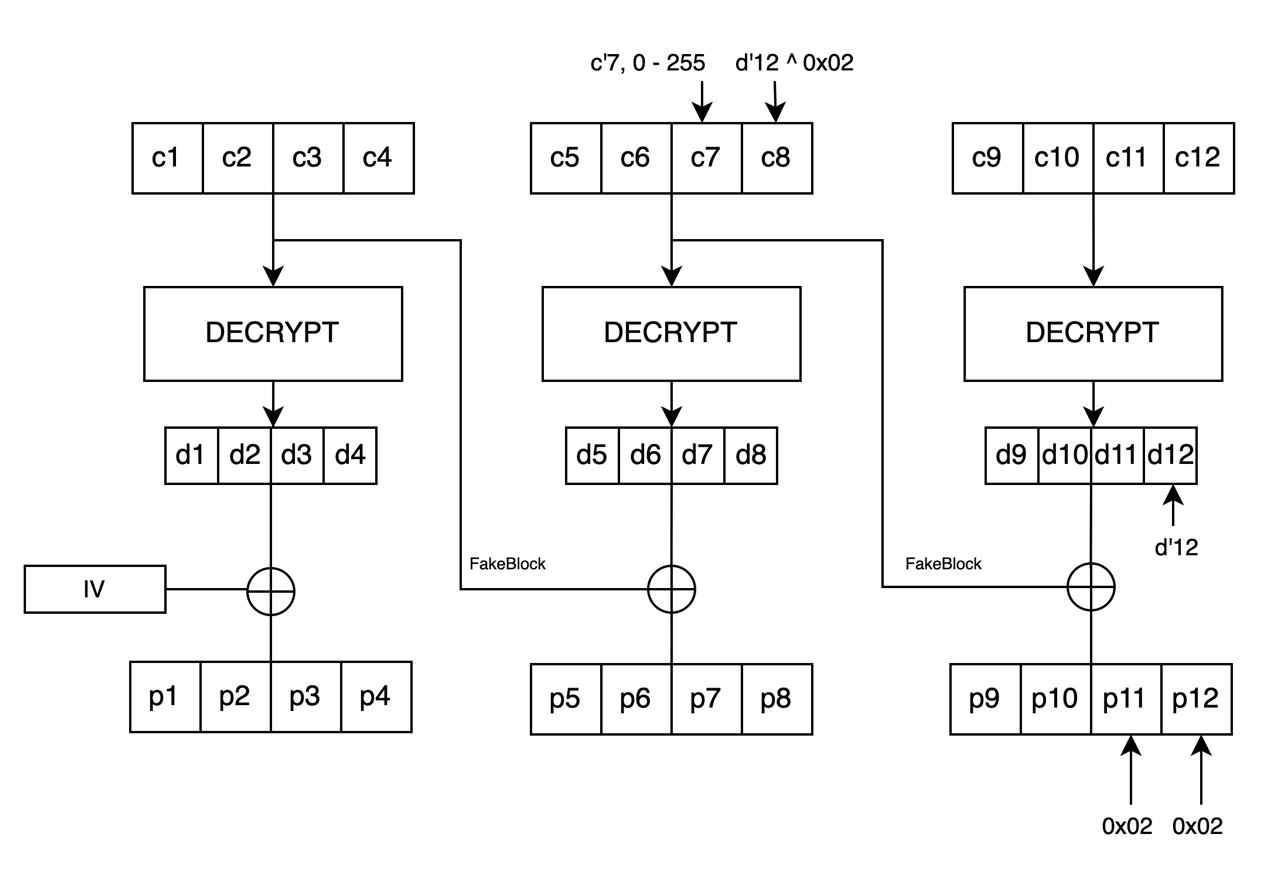
\includegraphics[width=0.8\textwidth]{img/attack_second_byte.jpeg}
    \centering
    \caption{Attacco al secondo byte}
    \label{fig:attack_3}
\end{figure}
\subsection{Blocchi Successivi}
\section{Prevenizone}